% ************ Chapter 2 ************
\chapter{Contexto} 
\label{cap:2}

\section{Estado da arte}
A empresa Natural Life iniciou a sua atividade como uma micro-empresa, tal tantas outras em Portugal, com apenas um software para a emissão de faturas e o acesso à plataforma de emissão de guias de transporte de resíduos. Todos os restante registos eram feitos à mão, sendo o seu tratamento igualmente feito por um processo manual o que levava a incongruências na informação registada além de muito tempo despendido no tratamento da informação.
No ano de 2015, como forma de baixar o impacto que esta metodologia tinha na gestão da empresa e até se encontrar uma solução capaz de satisfazer todas as necessidades da empresa, foi implementada uma solução com o software Microsoft Access.

\begin{figure}[ht] 
    \begin{center}
    % Requires \usepackage{graphicx}
    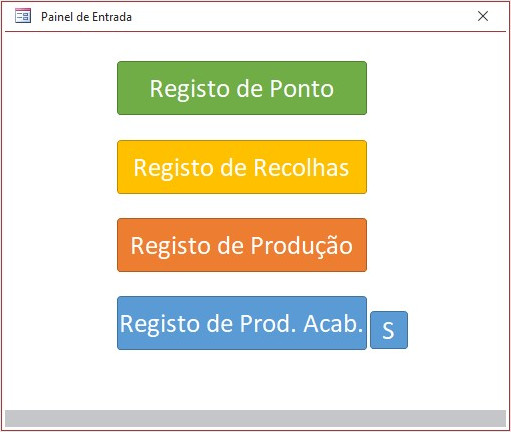
\includegraphics[width=0.75\textwidth,keepaspectratio]{figuras/AppAccess/0-MenuInicial.jpg}
    \caption{Menu inicial da aplicação embutida no Microsoft Access}\label{fig:app access home} 
    \end{center}
\end{figure}

A solução temporária cumpriu bem a sua função, havendo uma diminuição da informação mal apurada mesmo com a implementação de novos formulários de registo. A capacidade de desenhar os próprios formulários terá sido um dos fatores chave para o sucesso, visto que estes ponderam ser adaptados exatamente as necessidades da empresa. Ser completamente compatível com as aplicações Microsoft PowerBI e Microsoft Excel foi também uma característica decisiva no momento da opção pela plataforma. No entanto a plataforma Microsoft Access é bastante limitada, não sendo compatível, por exemplo, com o acesso em múltiplos terminais ao mesmo tempo ou precisar concluir o registo após o iniciar não sendo intuitivo o processo de cancelar o registo. Esta solução esta também limitada à plataforma Desktop, não sendo possível aceder em dispositivos movéis.


\section{Soluções já existentes}
No mercado, atualmente, já existem algumas soluções que poderiam ser implementadas neste caso. Dentre delas estão:

\begin{itemize}
    \item sage
    \item SAP
    \item Primavera
    \item Microsoft Dynamics
\end{itemize}

Todas são soluções aceites no mercado, mas todas elas são demasiado complexas para a realidade da empresa, tanto em termos de funcionalidades como em período de adaptação dos trabalhadores.
Além disto estas soluções exigiam a aquisição de licenças de software e infraestrutura TI\label{sym:TI} com custos não compatíveis com os planos de investimento da administração.

\section{Objetivo global}
Tendo em conta o que foi referido anteriormente, a administração optou pelo desenvolvimento de uma plataforma própria, cujo as características seriam definidas ao detalhe para que a plataforma fosse o mais adequado possível às necessidades da empresa.